% chktex-file 1 chktex-file 8

\tikzmath{
\dplunger     = 3;
\lplungertube = 5;
\dbarrel      = 1;
\lbarrel      = 6;
\ldead        = 1.5;
\ylowbarrel   = (\dplunger - \dbarrel)/2; 
\yhighbarrel  = \ylowbarrel + \dbarrel;
\xbarrelend   = \lplungertube + \ldead + \lbarrel;
\xbarrelstart = \lplungertube + \ldead;
\lproj        = 2;
\xproj        = \xbarrelstart + 1;
\xplungerheadstart = 1.5;
\lplungerhead      = 0.5;
\xplungerheadend   = \xplungerheadstart + \lplungerhead;
\ycenter = \dplunger/2;
\yfullspring = -\dplunger/2;
\yfullspringbelow = -7*\dplunger/8;
\yfullspringbelowbelow = -\dplunger;
\yfullspringabove = -\dplunger/4;
\halfyfullspringabove = -1*\dplunger/8;
\lfullspring = 7;
\ylbarrel = \ycenter + (\dplunger + \dbarrel)/4;
\xdead = \lplungertube + \ldead/2;
\xplungerheadunprimed = \lplungertube - \lplungerhead;
\yxz = \ycenter - (\dplunger + \dbarrel)/4;
\xdbarrel  = \xbarrelend - 1;
\xdplunger = \xplungerheadend + 1.0;
}

\begin{figure}
\centering
\begin{tikzpicture}
\draw[thick] (\xbarrelend, \yhighbarrel) -- (\lplungertube, \yhighbarrel) -- (\lplungertube, \dplunger) -- (0, \dplunger) -- (0, 0)         -- (\lplungertube, 0) -- (\lplungertube, \ylowbarrel) -- (\xbarrelend, \ylowbarrel);

\draw[thick,dashed] (\lplungertube, \ylowbarrel) -- (\lplungertube, \yhighbarrel);

\fill[fill=gray,draw=black,thick] (\xproj, \ylowbarrel) rectangle ++(\lproj, \dbarrel);

\fill[fill=gray,draw=black,thick] (\xplungerheadstart, 0) rectangle ++(\lplungerhead, \dplunger);

\tikzstyle{spring}=[thick,decorate,decoration={coil,amplitude=20,segment length=4pt}] % `zigzag` doesn't work right in LaTeXML, but `coil` does
\draw[spring] (0, \ycenter) -- (\xplungerheadstart, \ycenter);

\draw[<->,thick,fill=white] (\xbarrelstart, \ylbarrel) -- node[above] {$l_\text{travel}$} (\xbarrelend, \ylbarrel); % `fill=white` added to make the text fully visible in LaTeXML
\draw[thick,dashed] (\xbarrelend, \yhighbarrel) -- (\xbarrelend, \dplunger);

\node[draw=white] at (\xdead, \ycenter) {$V_\text{dead}$}; % `draw=white` added to make the text fully visible in LaTeXML

\draw[<->,thick] (\xplungerheadend, \halfyfullspringabove) -- node[below] {$y$} (\lplungertube, \halfyfullspringabove);
\draw[thick,dashed] (\lplungertube, \yfullspringabove) -- (\lplungertube, 0);
\draw[thick,dashed] (\xplungerheadend, \yfullspringabove) -- (\xplungerheadend, 0);

\draw[<->,thick] (\lplungertube, \ylbarrel) -- node[above] {$x_\text{0}$} (\xbarrelstart, \ylbarrel);
\draw[thick,dashed] (\xbarrelstart, \ylowbarrel) -- (\xbarrelstart, \dplunger);

\draw[<->,thick] (\lplungertube, \yxz) -- node[below] {$x$} (\xproj, \yxz);
\draw[thick,dashed] (\xproj, 0) -- (\xproj, \ylowbarrel);

\draw[<->,thick] (\xdbarrel, \ylowbarrel) -- node[right] {$d_\text{barrel}$} (\xdbarrel, \yhighbarrel);

\draw[<->,thick] (\xdplunger, \dplunger) -- node[right] {$d_\text{plunger}$} (\xdplunger, 0);
\end{tikzpicture}
\caption{Model spring blaster at arbitrary time as represented in BlasterSim.\label{fig:springer time zero}}
\end{figure}

\begin{figure}
\centering
\begin{tikzpicture}
\tikzstyle{spring_unprimed}=[thick,decorate,decoration={coil,amplitude=20,segment length=18pt}]
\tikzstyle{spring_full}=[thick,decorate,decoration={coil,amplitude=20,segment length=30pt}]
\draw[thick] (\xbarrelend, \yhighbarrel) -- (\lplungertube, \yhighbarrel) -- (\lplungertube, \dplunger) -- (0, \dplunger) -- (0, 0)         -- (\lplungertube, 0) -- (\lplungertube, \ylowbarrel) -- (\xbarrelend, \ylowbarrel);

\fill[fill=gray,draw=black,thick] (\xplungerheadunprimed, 0) rectangle ++(\lplungerhead, \dplunger);

\draw[spring_unprimed] (0, \ycenter) -- (\xplungerheadunprimed, \ycenter);

\draw[spring_full] (0, \yfullspring) -- (\lfullspring, \yfullspring); % has a long straight line segment in LaTeXML for some reason
\draw[<->,thick] (0, \yfullspringbelow) -- node[below] {$l_\text{spring}$} (\lfullspring, \yfullspringbelow);
\draw[thick,dashed] (0, \yfullspringbelowbelow) -- (0, 0);
\draw[thick,dashed] (\lfullspring, \yfullspringbelowbelow) -- (\lfullspring, 0);

\draw[<->,thick] (\lfullspring, \halfyfullspringabove) -- node[above] {$\Delta_\text{pre}$} (\xplungerheadunprimed, \halfyfullspringabove);
\draw[thick,dashed] (\xplungerheadunprimed, \yfullspringabove) -- (\xplungerheadunprimed, 0);
\end{tikzpicture}
\caption{Unprimed ($y = 0$) model spring blaster as represented in BlasterSim to show spring precompression.\label{fig:springer unprimed}}
\end{figure}

\begin{figure}
\centering
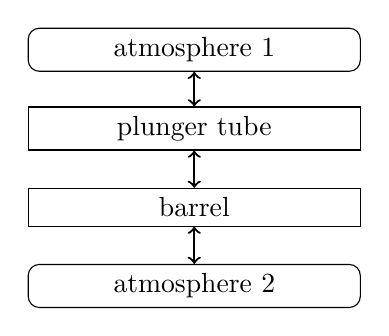
\begin{tikzpicture}
\tikzstyle{cv}       = [rectangle, minimum width=12em, text centered, draw=black]
\tikzstyle{cv_const} = [rectangle, rounded corners, minimum width=12em, text centered, draw=black]
\tikzstyle{arrow}    = [thick, <->]

\node (atm1)         [cv_const]                  {atmosphere~1};
\node (plunger tube) [cv, below of=atm1]         {plunger~tube};
\node (barrel)       [cv, below of=plunger tube] {barrel};
\node (atm2)         [cv_const, below of=barrel] {atmosphere~2};

\draw [arrow] (atm1)         -- (plunger tube);
\draw [arrow] (plunger tube) -- (barrel);
\draw [arrow] (barrel)       -- (atm2);
\end{tikzpicture}
\caption{Abstract connected control volume view of a springer blaster.\label{fig:springer control volumes}}
\end{figure}
